\documentclass[11pt]{article}
\usepackage[margin=1in]{geometry}
\usepackage{booktabs,graphicx,amsmath,amssymb,hyperref,xcolor,caption,microtype}
\emergencystretch=3em
\newcommand{\todo}[1]{\textcolor{red}{[TODO: #1]}}
\title{Beyond Disease Labels: Symptom-Based Vision-Language\\ Learning for Unseen Plant Diseases}
\author{Amirreza Zibafar \\ \small{Independent researcher} \\ \small{\texttt{amirzibafar1@gmail.com}}}
\date{}
\begin{document}
\maketitle

\begin{abstract}
Many crop diseases that matter to farmers, from regional diseases to pests and nutrient deficiencies, have no labelled image dataset, and annotating every disease is not realistic. Standard classifiers cannot help: they output a name from a fixed list. We take a different route and teach a model to act like an agronomist, who reads what is visible (which part is affected, its colour, texture, shape, pattern and density) and compares it with the known symptoms of candidate diseases, so that a new disease can be added with a text description instead of new training data. To our knowledge this is the first work that learns an image-to-symptom mapping from per-image symptom annotations and tests its transfer to diseases withheld from training. We provide symptom annotations (six attributes, 42 values) for 20{,}942 PlantWild photographs of 120 (crop, disease) units and a 10-fold evaluation in which every disease is held out once. A head trained on seen diseases predicts the symptoms of unseen diseases better than a same-crop prior for all six attributes and better than the global prior for affected part, shape and pattern. Our best model adapts both towers of SigLIP2-L with LoRA on re-sampled symptom descriptions. On held-out diseases it reaches 0.684 top-1 from symptom descriptions alone, ahead of CLIP-L/14 with disease names (0.495), a BCVSA-style baseline (0.456), a 7B vision-language model choosing among names (0.564) and the zero-shot SigLIP2-L it starts from (0.625); the gain over that start is $+0.059$ ($[+0.023, +0.092]$ over three seeds), and the correct disease is among its top three suggestions for 96\% of held-out diseases (chance 72\%). On 423 independent farmer photographs of 39 diseases the gains point the same way ($+0.02$ to $+0.03$) but are not yet statistically significant. Because the model scores readable symptom descriptions, its answers can be inspected and corrected by farmers or agronomists and a ranked shortlist of three can be offered when symptoms alone cannot separate diseases; correction by agronomists is left to future work.
\end{abstract}

\section{Introduction}
A farmer photographs a leaf with a problem that the diagnostic app has never been trained on. A conventional classifier must still answer with one of its known names, or fail. An agronomist would instead describe what is visible (brown, circular, scattered spots on the leaf) and compare it with what is known about candidate diseases. Our central hypothesis is that \emph{disease names are not transferable, but visual symptoms can provide a shared language for diagnosing diseases a model has never encountered} (Figure~\ref{fig:overview}). This paper tests that hypothesis; it does not assume it, and Section~\ref{sec:disc} separates what the experiments show from what they leave open.

\begin{figure}[t]\centering
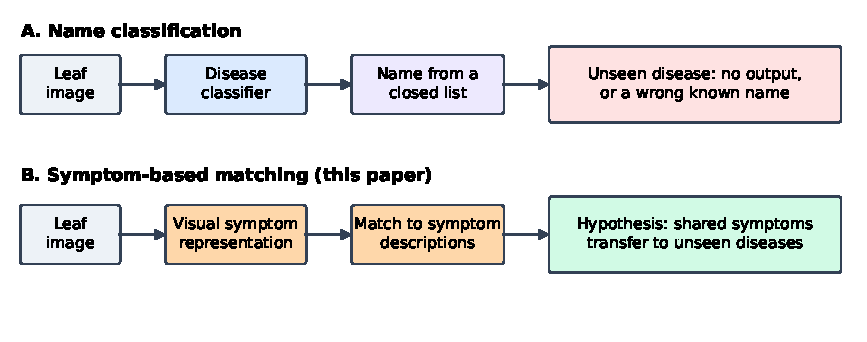
\includegraphics[width=\linewidth]{figures/fig_overview.pdf}
\caption{The problem and the proposed approach. A: a name classifier has no output for a disease outside its training list. B: images are mapped to symptoms and matched to descriptions of candidate diseases, so a new disease can be added as text. Panel B is a hypothesis; the experiments test it.}\label{fig:overview}
\end{figure}

We organise the paper around five questions. (Q1) Can symptoms of unseen diseases be predicted from images, and which attributes are learnable (Section~\ref{sec:transfer})? (Q2) Does vision-language adaptation help on held-out diseases (Sections~\ref{sec:results}, \ref{sec:textside}, \ref{sec:joint})? (Q3) Which description source transfers best: image-derived, blind LLM-written, or disease names (Sections~\ref{sec:sym}, \ref{sec:joint})? (Q4) Does internal performance carry over to farmer photographs (Section~\ref{sec:dg})? (Q5) Why do methods fail (Sections~\ref{sec:abl}, \ref{sec:limits})? A final question cuts across all of them: are we learning transferable symptoms, or information correlated with disease identity (Section~\ref{sec:disc})?

Most plant-disease recognition systems map an image to one of a fixed list of disease names. A disease outside the list cannot be predicted, and a model can score well by recognising the crop and the web source of an image rather than the lesion. Agronomists instead reason from symptoms: which plant part is affected, the colour and shape of lesions, their pattern. If a model learns to read those symptoms, a new disease described by its symptoms should be identifiable without retraining.

\textbf{Why this matters in practice.} Many problems that matter to farmers, such as nutrient deficiencies and pest damage, are poorly covered by public multi-crop image data (Section~\ref{sec:related}), and a classifier that outputs names from a fixed list has no output for them. A model that has learned what symptoms look like could in principle be given a text description of a new disorder and recognise it. Models trained on controlled images also lose accuracy in the field (99.35\% on held-out PlantVillage images against 31.4\% on images from online sources \cite{mohanty2016}), and early-stage recognition remains challenging \cite{xu2024}. Automatic plant disease identification is challenged by substantial variation in symptom appearance across disease developmental stages and by visual similarities between symptoms produced by different diseases \cite{barbedo2016}. This raises the possibility that models learning transferable symptom characteristics (colour changes, small lesions, spatial patterns on specific plant parts), rather than disease-specific appearance, could generalise better to early-stage manifestations. We present this as a hypothesis for future work, not a validated claim.
Our data contain one nutrient-deficiency unit and no growth-stage labels, so these two motivations are directions for future work and are not results of this paper (Section~\ref{sec:limits}).

We study this question in a controlled way. Our contributions are:
\begin{enumerate}
\item \textbf{A symptom-level annotation of plant disease images.} To our knowledge, the first multi-crop annotation of per-image visual symptoms: six attributes with 42 values for 20{,}942 PlantWild photographs of 120 (crop, disease) units, with documented provenance, quality limits and shortcut audits (Section~\ref{sec:data}). It is what makes it possible to learn symptoms on some diseases and test them on others, and we release it with the splits and code.
\item \textbf{A rigorous unseen-disease protocol.} A 10-fold unit-grouped cross-validation in which each disease is a test unit exactly once, validation units differ from test units, duplicates never cross splits, and an external farmer-photo test (DigiGreen) whose diseases are never trained on (Section~\ref{sec:eval}).
\item \textbf{Image-to-symptom transfer.} Attribute values learned on seen diseases are predicted for held-out diseases better than a same-crop prior for all six attributes, and better than the global prior for affected part, shape and pattern (Section~\ref{sec:transfer}).
\item \textbf{A joint vision+text LoRA model.} Adapting both SigLIP2 towers with re-sampled descriptions improves held-out-disease matching over zero-shot for image-derived, blind-description and blind-tag texts (three seeds, 10-fold CV; Section~\ref{sec:joint}); controls, earlier variants and a farmer-photo test are reported alongside.
\end{enumerate}

\section{Related Work}\label{sec:related}
\textbf{Prototype and zero-shot plant-disease recognition.} Wei et al.\ \cite{mvpdr} introduce the PlantWild benchmark and a baseline (MVPDR) that builds visual prototypes and text prototypes for PlantWild classes. Their ``zero-shot'' setting scores class text descriptions on the same classes that are used for training elsewhere, so it does not evaluate unseen diseases; PlantWild's text is written per class (from Wikipedia and an LLM), not per image. Snap'n Diagnose \cite{snapn} is a multimodal retrieval system built on PlantWild and MVPDR that accepts a photograph or a symptom text as the query. Zero-shot and generalised zero-shot plant-disease recognition has been studied with generic semantic embeddings and attributes \cite{kumar2024}, generative feature synthesis for unseen classes \cite{zhong2020}, vision-only unseen-pair learning \cite{chai2024}, and CLIP-style matching \cite{benabbas2025}. BCVSA \cite{bcvsa} is a publicly released bias-calibrated visual-semantic alignment framework for generalised zero-shot plant-disease recognition (a thesis project; we found no peer-reviewed paper), and we re-implement a BCVSA-style baseline. Vision-language and instruction-tuned models for agriculture, such as SCOLD \cite{scold}, AgroGPT \cite{agrogpt}, LeafNet \cite{leafnet}, and LLM-based diagnosis pipelines such as ChatLD \cite{chatld} and the symptom-knowledge agent SAGE \cite{sage}, use language for diagnosis. As far as we could determine, prior zero-shot plant-disease work either supplies attributes or text without learning a per-image symptom predictor, or evaluates unseen crop--disease combinations rather than whole diseases withheld from training: Kumar et al.\ \cite{kumar2024} feed 13 binary semantic attributes as input features and evaluate cross-crop splits whose disease labels are shared between training and test, ChatLD and SAGE prompt general-purpose vision-language models with disease descriptions without training \cite{chatld,sage}, and Chai et al.\ \cite{chai2024} study unseen crop--disease pairs from images alone. We are not aware of work that trains an image-to-symptom mapping on per-image symptom annotations and evaluates it on entire diseases withheld from training; we have not read Zhong et al.\ or Chai et al.\ in full. CLIP \cite{clip} and SigLIP~2 \cite{siglip2} provide the text--image matching these approaches rely on; classification by description \cite{cupl,menon2023} and attribute-based zero-shot learning \cite{lampert2014} motivate matching images to descriptions of properties instead of names.

\textbf{Dataset coverage beyond leaf-disease names.} Many problems that matter to farmers are poorly covered by public image data. PlantVillage \cite{mohanty2016,hughes2015} covers a small set of biotic leaf diseases of 14 crops under controlled conditions, and the datasets we know of that include other problem types are limited to one crop or region: CoLeaf-DB \cite{coleaf} (coffee nutrient deficiencies, photographed in a controlled setup), a maize nitrogen-deficiency set \cite{maizen} (one crop, field-trial canopy images), Paddy Doctor \cite{paddydoctor} (rice) and CCMT \cite{ccmt} (four crops in Ghana). Datasets of insect pests (IP102 \cite{ip102}) label the insect, not the damage it causes on the plant. To our knowledge there is no public multi-crop, in-the-wild dataset with many nutrient-deficiency or pest-damage \emph{symptom} classes: the nutrient datasets above are single-crop, and large multi-crop collections such as DLCPD-25 \cite{dlcpd} label mostly insect or mite species for pests; this is an argument from the datasets we examined, not a measured survey.

\textbf{Parameter-efficient adaptation.} We adapt SigLIP2 with LoRA \cite{lora}: first the vision tower with the text side fixed, then the text tower alone, and finally both towers jointly (Section~\ref{sec:joint}).

\textbf{Symptom-level supervision.} Among the benchmarks we examined, annotation beyond disease names is class-level, templated or small. PlantWild \cite{mvpdr} gives one text description per class; LeafNet \cite{leafnet} lists a symptom description per class in its metadata; PlantExpertVQA (first posted as PlantVillageVQA) \cite{pvvqa} and similar instruction datasets are generated from templates or metadata; PlantSeg \cite{plantseg} provides lesion masks without attribute text; and ADCG-18 \cite{zeng2024} attaches one free-text caption (colour, size, boundary) to each of 3{,}971 web images, which is the closest per-image resource we found but is small and unstructured. We are not aware of a benchmark with structured per-image symptom attributes across many crops, and we have not surveyed all benchmarks.

\section{Problem Formulation}
Let a disease unit $u$ be a (crop, disease) pair. Each image $x$ has a crop $c(x)$ and a unit $u(x)$. We split units, not images: a test unit never appears in training. At inference the crop is given, and the candidate set is every unit of that crop in the benchmark (seen and unseen), so a model that can only name seen diseases cannot score. Each unit has a text description $t_u$ built from tags. A model scores $s(x,u)=\langle f(x),g(t_u)\rangle$, where $f$ is the image tower, $g$ the text tower, and predicts $\arg\max_u s(x,u)$ over the candidates of $c(x)$. We distinguish two text tracks:
\begin{itemize}
\item \textbf{Symptom-only:} $t_u$ is a description generated from the unit's symptom tags and the crop word. No disease name appears in training or scoring.
\item \textbf{Symptom + name:} the score is the sum of the symptom-description logit and a disease-name prompt logit; names appear in training and scoring.
\end{itemize}
For an unseen disease the name route works only through what the pretrained text encoder already knows about the name, which is why we keep the two tracks separate.

\section{Dataset and Annotation}\label{sec:data}
\textbf{Source.} PlantWild \cite{mvpdr} photographs, filtered to the cleaned image set of our annotation version~3 (20{,}942 images, 120 disease units, 470 symptom clusters). Duplicate images (near-duplicate clusters) never cross splits. PlantWild is CC~BY-NC-ND and contains scraped web photos, so we release annotations, splits and scripts, not images.

\textbf{Annotation procedure.} Describing the visual symptoms of every image by hand is too costly, so the usual shortcut is to write one description per disease class (typically with an LLM) and give it to all images of the class. That shortcut is wrong whenever a disease shows different symptoms on different plant parts, which is common in our data: 66 of the 120 disease units affect more than one part (apple scab is annotated on fruit for 165 images and on leaf for 91; apple black rot on fruit, leaf and stem; apple rust on leaf, stem and fruit). We therefore annotate in three steps. (1) The \emph{affected part} is annotated for every image of the dataset and all of these labels were reviewed by the first author, so that symptoms can be defined for each (crop, disease, part) combination (244 combinations). (2) The images of each combination are split into a small number of groups of visually similar images (470 groups in total). The groups come partly from image-similarity clustering and partly from direct manual supervision with a cluster-review tool, in which outlier images were inspected and reassigned. (3) The remaining symptom tags (colour, texture, shape, pattern, lesion density) were then assigned to each group, for most groups by human annotators and for a smaller share by an LLM-assisted procedure; the released file marks which, with a lower confidence value for the latter. The annotators were the first author and a second annotator, who contributed a smaller share of the affected-part and symptom labels under the first author's supervision. An LLM (Claude) assisted throughout, mainly by suggesting which challenging images to examine and by proposing and phrasing tags, and later passes merged and split clusters and corrected tags. We do not claim the annotation is free of noise. It is, however, considerably more detailed than the class-level descriptions used in earlier work, and the source images are noisy too: PlantWild is collected from web searches and contains watermarked photos, charts and graphics, and images unrelated to the stated disease. Tags are group level: all images of a group share one tag set, so individual images may deviate from their group's tags. No inter-annotator agreement statistic was computed, so label reliability is not quantified beyond this. The annotations are released with the splits and code so that symptom transfer can be reproduced and extended.
The final vocabulary has 42 values after removing values at chance level in a preliminary audit (olive colour, hole shape, marginal-tip and vein-associated patterns, sticky-exudate texture) and dropping lesion size. A unit's text profile uses tags covering at least 25\% of its images.

\begin{figure}[t]\centering
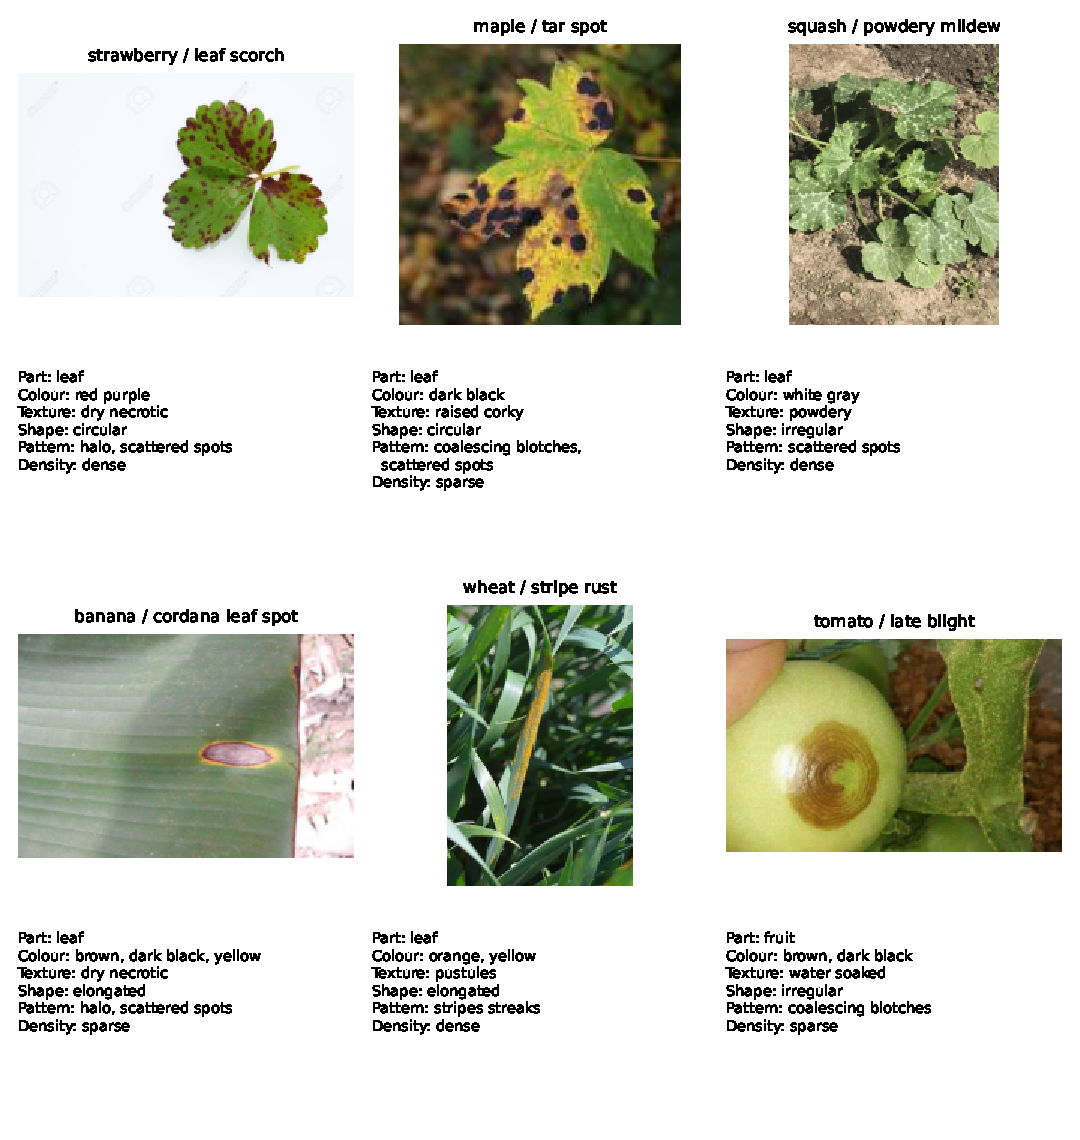
\includegraphics[width=\linewidth]{figures/annotation_examples.pdf}
\caption{Annotation examples (PlantWild photographs, annotations v3). We chose six units by eye whose tags visibly match the photo and whose symptoms differ, so these are good cases and not a random sample. Tags are assigned to groups of similar images, so an individual photo may deviate from its group's tags (here, for example, the wheat photo shows one stripe although the group density is dense), and attributes are not equally observable: part, colour and pattern are usually visible, texture and density often are not. Photographs are \copyright{} their PlantWild sources (CC BY-NC-ND) and are not covered by this paper's license.}\label{fig:examples}
\end{figure}

\textbf{Name-leakage audit.} Descriptions are built only from tag values and the crop word, so the disease name is never in the symptom text. Three vocabulary values also occur as words in disease names (\texttt{powdery}, \texttt{mosaic\_mottle}, \texttt{halo}); they are genuine symptom descriptors and were kept.

\section{Method}\label{sec:method}
We use SigLIP2-L (patch16, 256\,px) \cite{siglip2}. Text embeddings of unit and cluster descriptions are precomputed and fixed. In the first (vision-only) model, LoRA adapters (rank 16, on query/key/value/output projections of the vision tower; text tower frozen) are trained with a softmax cross-entropy over the same-crop \emph{training} units, with SigLIP2's own logit scale and bias, plus a cluster-level loss (weight 0.5). The step-0 model equals zero-shot retrieval because the adapter output starts at zero. Training images are sampled with weight inversely proportional to the square root of unit size. The final symptom-only setting trains 800 steps (batch 48, learning rate $2\times10^{-5}$) with long and tag description styles; the name track trains 400 steps (learning rate $5\times10^{-5}$) with long, tag and name styles and scores description plus name. The checkpoint step is chosen on validation units, which are disjoint from test units. Section~\ref{sec:joint} describes the final joint vision+text variant, which adapts both towers.

\begin{figure}[t]\centering
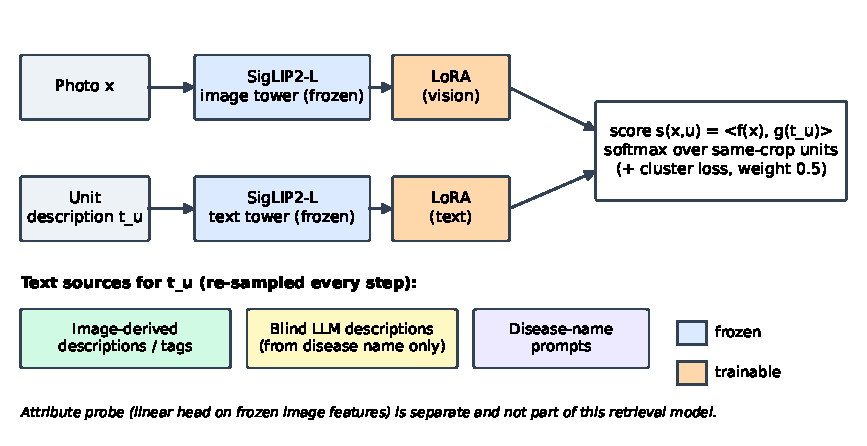
\includegraphics[width=\linewidth]{figures/fig_architecture.pdf}
\caption{Joint model. Blue: frozen pretrained weights; orange: trainable LoRA adapters (vision tower only, text tower only, or both in the joint model). Text sources for training and scoring: image-derived descriptions, blind LLM descriptions and tag lists, and disease-name prompts. The attribute probe (Section~\ref{sec:transfer}) is a separate linear head on frozen image features and is not part of this retrieval model.}\label{fig:arch}
\end{figure}

\section{Evaluation Protocol and Baselines}\label{sec:eval}
\textbf{10-fold unit-grouped CV.} The 120 units are divided into 10 folds of 12 balanced by tag novelty, crop spread and image count. For fold $k$, units in fold $k$ are test, units in fold $k{+}1$ are validation, the rest train; healthy photos are fixed 60/20/20 per crop. Four crops with a single disease unit (maple, squash, basil, onion) have a candidate set of one and are excluded from the headline, leaving 116 test units. The metric is top-1 accuracy averaged over test units (unit-macro) with crop given. Uncertainty is a bootstrap over folds (10{,}000 resamples); trained models use three seeds.

\begin{figure}[t]\centering
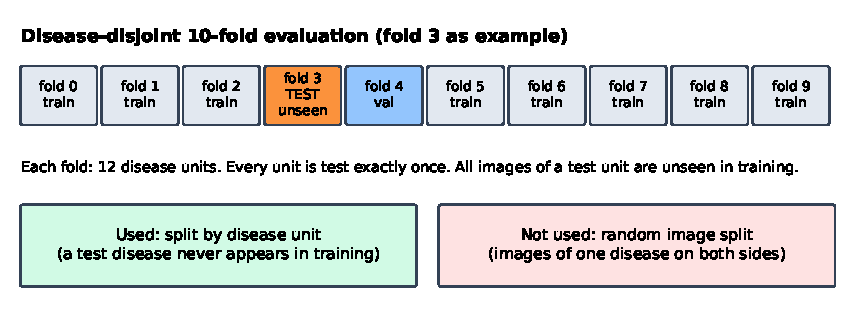
\includegraphics[width=\linewidth]{figures/fig_split.pdf}
\caption{Disease-disjoint evaluation. The 120 units are split into 10 folds. For fold $k$, fold $k$ is test, fold $k{+}1$ is validation and the others train. Duplicates never cross splits.}\label{fig:split}
\end{figure}

\textbf{Caveat.} In the CV, the text profile of a held-out disease is built from the tags of its own images, which is optimistic compared with a profile written by an expert for a new disease. The external DigiGreen test avoids this: its images are scored against profiles built from PlantWild photographs of the matched disease.

\textbf{External test.} DigiGreen \cite{digigreen} is a public set of 989 farmer-submitted crop photographs (74 crops, mostly from India) with agronomist annotations; we use 14 disease types matched to PlantWild units (near-duplicates of PlantWild removed), 69 main images; these diseases are excluded from training. No validation set is available, so the final training step is used.

\textbf{Blind profiles.} To remove the caveat above, an open LLM (Qwen2.5-VL-7B-Instruct used text-only) writes a symptom profile for every disease from the crop and disease name only, restricted to our tag vocabulary. It sees neither images nor our annotations. We score held-out diseases with these blind profiles in the CV and for DigiGreen diseases that have no PlantWild annotation. Agreement with our image-derived tags (any overlap of values, 120 PlantWild units): affected part 0.93, colour 0.88, texture 0.58, shape 0.61, pattern 0.58, lesion density 0.27.

\textbf{Large DigiGreen test.} All single-diagnosis, non-healthy DigiGreen images whose diagnosis has at least three images and whose crop has at least two such diagnoses: 423 images, 39 disease types, 12 crops (DigiGreen crop names are mapped to PlantWild names where they differ, e.g. maize to corn). Candidates are the DigiGreen types of the crop (a variant adds the crop's PlantWild units as extra distractors). A model is trained on PlantWild with every unit that matches any DigiGreen disease removed (matched by crop and normalised disease name; 34 of the 39 types have no counterpart), three seeds, final step. Scores use blind profiles; no DigiGreen label or image is used for training or for profile writing.

\textbf{Baselines (re-run on identical splits).} Chance; crop prior (image-independent); nearest seen disease profile; linear tag heads with profile lookup; CLIP-L/14 zero-shot with name prompts; a BCVSA-style blend of DINOv2-L \cite{dinov2} features aligned to CLIP text and CLIP zero-shot (our re-implementation, two encoders); a Qwen2.5-VL-7B \cite{qwen} zero-shot symptom tagger with profile lookup and a Qwen2.5-VL-7B multiple-choice-by-name run (both on a fixed sample of up to 6 test images per unit, $\dagger$); SigLIP2-L zero-shot with description, name and description+name prompts. Shuffling controls permute unit texts within a crop.

\section{Results}\label{sec:allresults}
We answer the questions of the introduction in turn: baselines and the effect of adaptation (Sections~\ref{sec:results}, \ref{sec:textside}, \ref{sec:joint}), whether symptoms of unseen diseases can be read (Section~\ref{sec:transfer}), which description source transfers (Section~\ref{sec:sym}), and whether the gains carry over to farmer photographs (Section~\ref{sec:dg}). The joint vision+text model of Section~\ref{sec:joint} is our final model; the earlier subsections are the steps that lead to it.

\subsection{Baselines and vision-only adaptation}\label{sec:results}
\begin{table}[t]\centering\small
\resizebox{\linewidth}{!}{\begin{tabular}{lc}\toprule Method & Top-1 (unit-macro)\\\midrule
Chance (1/\#candidates) & 0.267\\
Crop prior (no image) & 0.009\\
Nearest seen disease profile & 0.000\\
Linear tag head + profile lookup & 0.361\\
BCVSA-style blend (DINOv2-L + CLIP-L/14) & 0.456\\
CLIP-L/14 zero-shot, names & 0.495\\
Qwen2.5-VL-7B tags + lookup$^\dagger$ & 0.275\\
Qwen2.5-VL-7B multiple choice, names$^\dagger$ & 0.564\\
SigLIP2-L zero-shot, description & 0.627\\
SigLIP2-L zero-shot, name & 0.639\\
SigLIP2-L zero-shot, description + name & 0.683\\
Ours, symptom text only (3 seeds) & 0.645\\
Ours, symptom text + name (3 seeds) & 0.707\\
\bottomrule\end{tabular}
}
\caption{Unit-macro top-1 on the 10-fold unit-grouped CV (116 test units, crop given). Trained models: mean of three seeds. $^\dagger$ evaluated on a sample of up to 6 test images per unit. The tag-head row is the single-run number from our experiment log. ``Ours'' is the vision-only LoRA model; the final joint vision+text model (0.684 with image-derived descriptions, compared with 0.625 for its own zero-shot start) is in Table~\ref{tab:joint}.}
\label{tab:main}
\end{table}

Table~\ref{tab:main} gives the comparison. Supervised symptom-only training reaches 0.645 against 0.625 for zero-shot description retrieval (seeds 0.646, 0.633, 0.655; $+0.019$, 95\% interval $[-0.010, 0.049]$; improved on 5 of 10 folds), a gain that the fold-level interval does not separate from zero. The name-augmented model reaches 0.707 against 0.680 (seeds 0.708, 0.704, 0.709; $+0.027$, $[0.006, 0.049]$; 7 of 10 folds). Figure~\ref{fig:folds} shows the gain is uneven across folds: it is clear on some folds and absent or negative on others. All re-implemented published-style baselines are below the SigLIP2 zero-shot reference. Caveat: these are our re-implementations on our splits; they are not reproductions of the original papers' numbers.

\begin{figure}[t]\centering
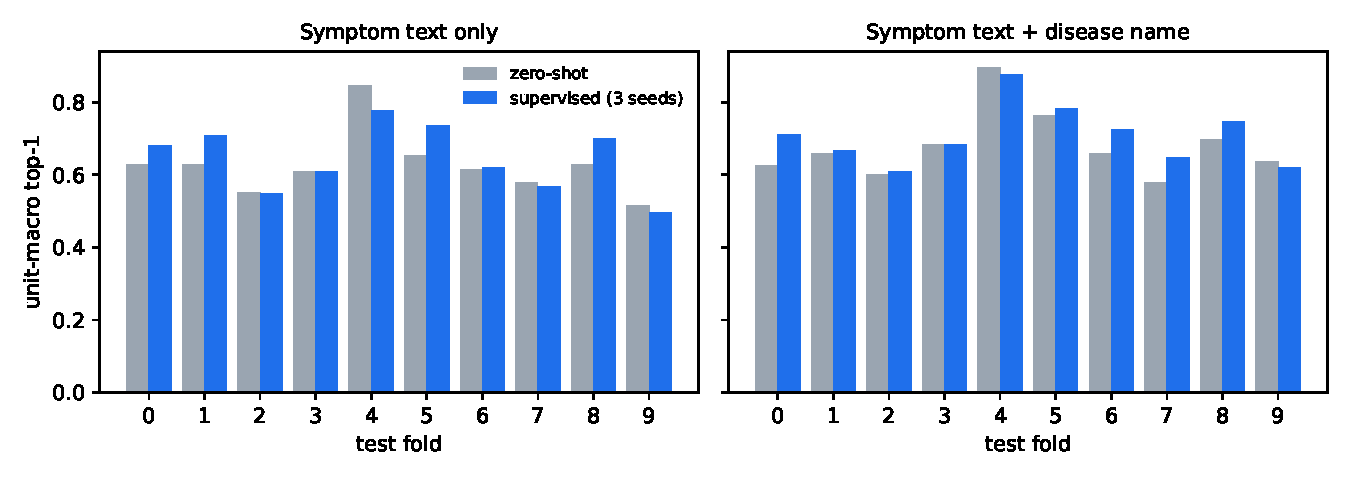
\includegraphics[width=0.95\linewidth]{figures/per_fold.pdf}
\caption{Per-fold unit-macro top-1, zero-shot versus supervised (mean of three seeds).}\label{fig:folds}
\end{figure}

\subsection{Reading the symptoms of unseen diseases}\label{sec:transfer}
The question this work is built around is whether a model that has seen the symptoms of some diseases can describe the symptoms visible in a photograph of a disease it has never seen. Matching an image to a symptom \emph{text} (Sections~\ref{sec:results}--\ref{sec:dg}) tests this only indirectly, because the text of the held-out disease has to be right as well. Here we test the image-to-symptom direction directly.

\textbf{Setup.} We train one linear head per attribute on frozen SigLIP2-L-256 image features of the training diseases (soft cross-entropy over the attribute's values, target uniform over the values annotated for the image's group, diseases balanced by $1/\sqrt{n}$, epoch chosen on the validation diseases) and apply it to the images of the held-out diseases of the 10-fold CV. A prediction counts as a hit if the top value is among the annotated values of the image's group; scores are macro-averaged over test diseases and intervals are bootstrap over folds. We compare with (i) zero-shot scoring of generic value prompts, (ii) the value that is most common among all training images, and (iii) the most common value among training images of the same crop, which is the shortcut available to any model that recognises the crop. Labels are group level, so a hit means ``consistent with the annotated look of the group'', not ``correct for this specific image''.

\begin{table}[t]\centering\small
\resizebox{\linewidth}{!}{\begin{tabular}{lcccccc}\toprule Attribute & Zero-shot prompts & Most common & Same-crop prior & Trained head & Head $-$ crop prior & Head $-$ most common\\\midrule
Affected part & 0.724 & 0.715 & 0.619 & 0.931 & +0.312 [+0.250, +0.373] & +0.216 [+0.164, +0.273]\\
Colour & 0.600 & 0.696 & 0.554 & 0.700 & +0.146 [+0.055, +0.235] & +0.004 [-0.057, +0.067]\\
Texture & 0.344 & 0.653 & 0.434 & 0.660 & +0.226 [+0.128, +0.322] & +0.007 [-0.068, +0.087]\\
Shape & 0.391 & 0.424 & 0.268 & 0.580 & +0.312 [+0.229, +0.387] & +0.156 [+0.078, +0.226]\\
Pattern & 0.501 & 0.248 & 0.256 & 0.552 & +0.297 [+0.232, +0.360] & +0.304 [+0.214, +0.384]\\
Lesion density & 0.163 & 0.483 & 0.471 & 0.550 & +0.079 [+0.024, +0.129] & +0.067 [-0.058, +0.190]\\
\bottomrule\end{tabular}
}
\caption{Image-to-symptom transfer to held-out diseases (10-fold CV, one seed). Fraction of test images whose top predicted value is among the annotated values of their group, macro over diseases. The trained head is a linear layer on frozen image features trained on seen diseases only. Differences are with bootstrap 95\% intervals over folds.}\label{tab:transfer}
\end{table}

\textbf{Results.} The trained head beats the same-crop prior on all six attributes (differences $+0.08$ to $+0.31$, intervals above zero), so the transfer is not explained by recognising the crop. Against the stronger global baseline it improves clearly for the affected part ($+0.216$), shape ($+0.156$) and pattern ($+0.304$), and ties it for colour, texture and lesion density, where one value dominates the labels. Zero-shot prompts, in contrast, fall below the prior for texture (0.344), lesion density (0.163) and colour, so reading these attributes from the image is not something the pretrained model does with generic prompts but something that is learned from the training diseases and carries over to unseen ones. This is the evidence we consider closest to the claim of the paper, and its limits are the group-level labels, the single seed, the coarse ``top-1 in annotated set'' hit and the fact that a linear head on frozen features, not the text-matching model, is evaluated.

\subsection{Description sources, controls and attribute probes}\label{sec:sym}
\textbf{Controls on text.} Shuffling the description or the name text across diseases of the same crop reduces zero-shot top-1 from 0.627 and 0.639 to 0.136 and 0.126; this control never leaves a disease with its own text, so it falls below chance (0.267) by construction, and shows that scores depend on the text matching the correct disease. Image-independent baselines (crop prior, nearest seen profile) score about zero because they can only point to diseases seen in training. Restricting candidates to unseen diseases lets the same two baselines reach 0.853 and 0.874, because each crop then has about one unseen candidate; this is a benchmark diagnostic, not a competitor.

\textbf{Shuffled-label control for the supervised model.} We train with the same recipe but with the unit labels of the training images deranged within each crop (no cluster loss). The validation-based step selection chose step 0, i.e. no gain, in all 10 folds. Without selection, the final-step model scores 0.199 against 0.625 for zero-shot, so the training labels carry the signal and the gain of the real model is not an artefact of the training procedure.

\textbf{Profiles written blind.} Table~\ref{tab:blind} re-scores the same checkpoints with different texts for the held-out diseases. With profiles written blind by an LLM, zero-shot accuracy is 0.563 instead of 0.625, and the supervised model gives no gain (0.563). The gain in the main table therefore depends on how the held-out profile is produced: it appears with profiles built from the tags of the held-out images (the style the model was trained on) and not with LLM-written profiles in the same template.
\begin{table}[t]\centering\small
\resizebox{\linewidth}{!}{\begin{tabular}{lcccc}\toprule Text used to score a held-out disease & Zero-shot & Supervised & Gain [95\% CI] & Folds improved\\\midrule
Image-derived profile (tag shares), description & 0.625 & 0.646 & +0.020 [-0.010, 0.051] & 5/10\\
Blind LLM profile, description & 0.563 & 0.563 & -0.000 [-0.027, 0.028] & 4/10\\
Blind LLM profile, tag list & 0.490 & 0.510 & +0.020 [-0.010, 0.049] & 5/10\\
Disease-name prompt & 0.639 & 0.630 & -0.009 [-0.030, 0.010] & 4/10\\
\bottomrule\end{tabular}
}
\caption{PlantWild 10-fold CV, same fine-tuned checkpoints (seed 0, 10 folds), different texts for held-out diseases. Unit-macro top-1; interval is a bootstrap over folds. The model was trained with image-derived profiles of training diseases (description and tag styles).}\label{tab:blind}
\end{table}

\textbf{Training on blind profiles.} The mismatch between training text (image-derived) and test text (LLM-written) may explain the missing gain, so we also trained with the blind LLM profiles of the training diseases, with model selection on the blind profiles of the validation diseases (Table~\ref{tab:blindtrain}; one seed, 10 folds). Scoring with blind profiles now gains +0.022 for the description (interval $[0.002, 0.044]$, 6 of 10 folds) and +0.047 for the tag list ($[0.021, 0.072]$, 7 of 10). This is a modest improvement over zero-shot, and it is the setting that matches deploying the model for a disease described only by text. The gain does not carry to the external test (Section~\ref{sec:dg}).
\begin{table}[t]\centering\small
\resizebox{\linewidth}{!}{\begin{tabular}{lccc}\toprule Text used to score a held-out disease & Zero-shot & Blind-trained & Gain [95\% CI] (folds improved)\\\midrule
Blind LLM profile, description & 0.563 & 0.585 & +0.022 [0.002, 0.044] (6/10)\\
Blind LLM profile, tag list & 0.490 & 0.537 & +0.047 [0.021, 0.072] (7/10)\\
Disease-name prompt & 0.639 & 0.634 & -0.005 [-0.028, 0.020] (3/10)\\
Image-derived profile, description & 0.625 & 0.636 & +0.011 [-0.012, 0.034] (4/10)\\
\bottomrule\end{tabular}
}
\caption{PlantWild 10-fold CV, models trained and selected on blind LLM profiles (seed 0). Unit-macro top-1; bootstrap interval over folds.}\label{tab:blindtrain}
\end{table}

\textbf{Per-attribute probe.} For each test image we score the vocabulary values of one attribute with generic prompts (e.g.\ ``a photo of a plant with brown lesions'') and check whether the top value is among the annotated values of the image's group (Table~\ref{tab:attr}). The supervised model improves clearly over zero-shot and over a train-set prior only for the affected plant part (0.818 against 0.724 and 0.755). For colour, shape and pattern it is at or below the prior, and for texture and lesion density it is far below it. The prior is strong because the tag distribution is skewed, and the probe prompts are crude, so this analysis is limited; but it gives no support for the claim that this vision-only model has learned colour, texture, pattern or density. Table~\ref{tab:jointattr} gives the same probe for the final joint model.
\begin{table}[t]\centering\small
\resizebox{\linewidth}{!}{\begin{tabular}{lccccc}\toprule Attribute & Zero-shot & Supervised & Train-set prior & Chance\\\midrule
Affected part & 0.724 & 0.818 & 0.755 & 0.129\\
Colour & 0.599 & 0.644 & 0.655 & 0.294\\
Texture & 0.308 & 0.293 & 0.614 & 0.166\\
Shape & 0.405 & 0.425 & 0.410 & 0.170\\
Pattern & 0.530 & 0.532 & 0.543 & 0.205\\
Lesion density & 0.129 & 0.233 & 0.535 & 0.335\\
\bottomrule\end{tabular}
}
\caption{Per-attribute probe on test images (mean over the 10 folds, seed 0). Fraction of images whose top-scoring value is among their group's annotated values, averaged over test \emph{images} (not diseases); prior = most frequent individual training value; chance = expected hit of a random value. The numbers are therefore not comparable with the disease-macro Tables~\ref{tab:transfer} and~\ref{tab:jointattr}.}\label{tab:attr}
\end{table}

The probe above uses zero-shot value prompts and is averaged over images. Section~\ref{sec:transfer} instead trains a head on the training diseases and finds that it does transfer for several attributes, so the weak result here is a property of generic prompts with a frozen model, not of the image features.

\subsection{Adapting the text tower}\label{sec:textside}
So far only the vision tower was adapted. Because the held-out diseases are specified by text, we also adapted the text side, on cached frozen image features so that many variants and seeds are affordable. Descriptions are re-sampled at every step from the unit's profile (attribute dropout, subsets of multi-valued attributes, five templates) and from both profile sources (image-derived and blind LLM), so the encoder cannot memorise fixed strings. Model selection uses validation diseases, and held-out diseases are scored with the canonical templates.

\begin{table}[t]\centering\small
\resizebox{\linewidth}{!}{\begin{tabular}{lcccc}\toprule Text-side model & Image-derived description & Blind description & Blind tag list & Name prompt\\\midrule
Text LoRA, no hard negatives (3 seeds) & +0.031 [-0.006, +0.063] & +0.031 [+0.002, +0.057] & +0.075 [+0.043, +0.117] & +0.008 [-0.011, +0.026]\\
Text LoRA + hard negatives & +0.013 [-0.026, +0.048] & +0.005 [-0.050, +0.047] & +0.041 [+0.006, +0.081] & -0.004 [-0.026, +0.018]\\
Text LoRA, blind profiles only + hard neg. & -0.055 [-0.111, -0.006] & -0.008 [-0.051, +0.021] & +0.025 [-0.002, +0.054] & -0.011 [-0.050, +0.027]\\
Last 4 text layers + hard negatives & -0.018 [-0.054, +0.013] & -0.012 [-0.072, +0.030] & +0.004 [-0.036, +0.047] & -0.020 [-0.049, +0.009]\\
Last 4 text layers, no hard negatives & +0.003 [-0.037, +0.048] & +0.031 [-0.005, +0.068] & +0.052 [-0.002, +0.113] & -0.000 [-0.026, +0.024]\\
mpnet + projection & -0.021 [-0.057, +0.007] & -0.023 [-0.065, +0.021] & -0.025 [-0.074, +0.021] & -0.015 [-0.051, +0.016]\\
mpnet last 2 layers + projection & -0.027 [-0.066, +0.011] & -0.000 [-0.043, +0.042] & -0.013 [-0.056, +0.036] & -0.017 [-0.052, +0.014]\\
\bottomrule\end{tabular}
}
\caption{Text-side adaptation, PlantWild 10-fold CV: gain over the same run's step 0 (zero-shot) in unit-macro top-1, with bootstrap 95\% intervals over folds. First row is the mean of 3 seeds, the others one seed.}\label{tab:textside}
\end{table}

\textbf{LoRA on the text tower helps most.} Averaged over 3 seeds, it raises the blind tag-list score from 0.493 to 0.568 ($+0.075$, $[+0.043, +0.117]$, better in 10 of 10 folds) and the blind description from 0.561 to 0.592 ($+0.031$, $[+0.002, +0.057]$), larger than the vision-LoRA gains of Section~\ref{sec:sym}. The gain for image-derived descriptions ($+0.031$) and for name prompts ($+0.008$) is within noise. \textbf{Hard negatives hurt.} Adding one-attribute-swapped copies of each description as negatives reduces the gain (blind description $+0.031 \to +0.005$; last-layers variant $+0.031 \to -0.012$), probably because swapping one value often yields a valid description of another disease. \textbf{Unfreezing the last text layers} does not improve over LoRA. \textbf{Other text encoders} (all-mpnet-base-v2, either frozen with a projection distilled to the SigLIP text space or with its last layers trained) give no gain over their own starting point, which is below SigLIP's text tower (name prompts 0.438 against 0.639), and blending their scores with SigLIP adds at most 0.02. \textbf{Free-text LLM paraphrases.} Averaging six blind LLM paraphrases per disease, with no training, scores 0.409 against 0.562 for the structured blind profile (difference $-0.154$, $[-0.233, -0.076]$); combining paraphrases with tags and name reaches 0.618, which stays below the name prompt alone (0.639). We did not run the other sentence encoders we downloaded (bge, e5, PubMedBERT), because the two variants above showed no gain.

\begin{table}[t]\centering\small
\resizebox{\linewidth}{!}{\begin{tabular}{lcccc}\toprule Text (39 types) & Zero-shot & Text LoRA (3 seeds) & Gain over types [95\% CI] & Better / worse\\\midrule
Blind description & 0.395 & 0.424 & +0.029 [-0.028, +0.086] & 14 / 12\\
Blind tag list & 0.391 & 0.420 & +0.029 [-0.046, +0.106] & 18 / 11\\
Disease name & 0.476 & 0.463 & -0.013 [-0.046, +0.019] & 12 / 11\\
\bottomrule\end{tabular}
}
\caption{Large DigiGreen test (423 images, 39 types, blind profiles). Text LoRA trained on all PlantWild diseases that do not match a DigiGreen type (3 seeds, 250 steps) against the zero-shot score of the same pipeline. Gain with bootstrap interval over types.}\label{tab:dgtext}
\end{table}

\textbf{External test.} On the large DigiGreen test the text-LoRA gain is positive but not significant (Table~\ref{tab:dgtext}: $+0.029$ for the description and the tag list, intervals include zero; 14 types better and 12 worse for descriptions). We therefore report the text-side gain as a cross-validation result that is not yet confirmed on external farmer photographs.

\subsection{Joint vision and text adaptation}\label{sec:joint}
The text-tower and vision-tower experiments above each change one side. Here both towers carry LoRA adapters (rank 16; learning rate $2\times10^{-5}$ for the vision tower and $10^{-4}$ for the text tower) and are trained together end to end: images are encoded with gradients, and descriptions of the training diseases are re-sampled at every step from both profile sources (image-derived and blind LLM; attribute dropout, value subsets, five templates), with a softmax over same-crop training units. The adapters start at zero, so step 0 is the zero-shot model, and the checkpoint step is chosen on validation diseases (600 steps at most; one fold selected step 0, i.e.\ no change). Held-out diseases are scored with the canonical templates. Three seeds, 10 folds; gains are seed-averaged per fold with bootstrap intervals over folds.

\begin{table}[t]\centering\small
\resizebox{\linewidth}{!}{\begin{tabular}{lcccc}\toprule Joint model (3 seeds) & Image-derived description & Blind description & Blind tag list & Name prompt\\\midrule
Zero-shot & 0.625 & 0.561 & 0.490 & 0.638\\
Vision + text LoRA & 0.684 (+0.059 [+0.023, +0.092]) & 0.609 (+0.048 [+0.011, +0.083]) & 0.582 (+0.092 [+0.053, +0.136]) & 0.656 (+0.018 [-0.008, +0.043])\\
\bottomrule\end{tabular}
}
\caption{Joint vision+text LoRA, PlantWild 10-fold CV, unit-macro top-1 (mean of three seeds); in brackets the gain over the same run's zero-shot start with a bootstrap 95\% interval over folds.}\label{tab:joint}
\end{table}

\textbf{Results.} Table~\ref{tab:joint} shows gains for all three description types: $+0.059$ for image-derived descriptions (better in 8 of 10 folds, worse in 1), $+0.048$ for blind descriptions (7 better, 2 worse) and $+0.092$ for blind tag lists (9 better, 0 worse); intervals exclude zero. Per-seed gains are $0.056$, $0.065$, $0.057$ (image-derived), so the seeds agree. The gains are larger than for text-only LoRA ($+0.031$, $+0.031$, $+0.075$; the image-derived gain of that variant had an interval including zero) and than for vision-only training ($+0.02$ to $+0.05$). Name prompts improve by $+0.018$ ($[-0.008, +0.043]$), so the model does not simply improve its handling of disease names. We did not run a matched compute comparison, and the three variants differ in training details, so the ranking is indicative.

\begin{table}[t]\centering\small
\resizebox{\linewidth}{!}{\begin{tabular}{lcccc}\toprule Text (39 types, 3 seeds) & Zero-shot & Joint LoRA & Gain over types [95\% CI] & Better / worse\\\midrule
Blind description & 0.395 & 0.421 & +0.026 [-0.041, +0.092] & 14 / 11\\
Blind tag list & 0.392 & 0.410 & +0.018 [-0.064, +0.100] & 17 / 12\\
Disease name & 0.479 & 0.507 & +0.028 [-0.031, +0.088] & 17 / 14\\
\bottomrule\end{tabular}
}
\caption{Joint model on the large DigiGreen test (423 images, 39 types, blind profiles), trained on PlantWild diseases that do not match a DigiGreen type (400 steps, final step, three seeds); gain with bootstrap interval over types.}\label{tab:jointdg}
\end{table}

\textbf{External test.} On the large DigiGreen test the joint model gains $+0.026$ for blind descriptions, $+0.018$ for tag lists and $+0.028$ for disease names (Table~\ref{tab:jointdg}); all intervals include zero, and name prompts remain better than symptom descriptions in absolute terms (0.507 against 0.421). The cross-validation result is therefore not confirmed on independent farmer photographs at this sample size.

\textbf{Per-attribute reading.} We repeat the per-attribute test with the adapted models, using the disease-macro hit criterion and priors of Section~\ref{sec:transfer} and the generic value prompts of Section~\ref{sec:sym}, scored with the adapted text tower (10 folds; joint model: mean over three seeds; vision-only model: one seed; Table~\ref{tab:jointattr}). Against the same-crop prior the joint model is better for affected part ($+0.159$), shape ($+0.197$) and pattern ($+0.273$), with intervals above zero. Against the stronger global prior it is better for affected part ($+0.063$, $[+0.012, +0.112]$) and pattern ($+0.281$), indistinguishable for shape and colour, and clearly worse for texture ($-0.340$) and lesion density ($-0.312$), where the generic prompts are poor and the annotated values are dominated by one value. Relative to its own zero-shot start the gain is significant for part ($+0.054$), colour ($+0.034$) and shape ($+0.073$) and not for pattern, texture or density. The vision-only model shows the same picture and is not worse: it is better than the joint model for affected part ($0.818$ against $0.778$, $+0.103$ over the global prior) and lesion density ($0.261$ against $0.171$, still below the prior), slightly worse for shape and pattern, and the differences between the two models are small relative to the fold intervals. Hence the larger matching gain of the joint model is not explained by a better reading of generic attribute prompts; it presumably comes from adapting the text tower to the description templates, which we did not test in isolation. Both models read affected part and pattern better than any prior, and neither reads texture or lesion density with these prompts.
\begin{table}[t]\centering\small
\resizebox{\linewidth}{!}{\begin{tabular}{lccccccc}\toprule Attribute & Global prior & Same-crop prior & Zero-shot prompts & Vision-only (1 seed) & Joint (3 seeds) & Vision-only $-$ prior & Joint $-$ prior\\\midrule
Affected part & 0.715 & 0.619 & 0.724 & 0.818 & 0.778 & +0.103 [+0.067, +0.139] & +0.063 [+0.012, +0.112]\\
Colour & 0.696 & 0.554 & 0.603 & 0.629 & 0.637 & -0.067 [-0.146, +0.008] & -0.059 [-0.140, +0.012]\\
Texture & 0.653 & 0.434 & 0.341 & 0.333 & 0.313 & -0.321 [-0.469, -0.165] & -0.340 [-0.466, -0.195]\\
Shape & 0.424 & 0.268 & 0.393 & 0.421 & 0.465 & -0.003 [-0.084, +0.088] & +0.041 [-0.028, +0.125]\\
Pattern & 0.248 & 0.256 & 0.501 & 0.505 & 0.529 & +0.256 [+0.170, +0.332] & +0.281 [+0.200, +0.350]\\
Lesion density & 0.483 & 0.471 & 0.165 & 0.261 & 0.171 & -0.222 [-0.333, -0.095] & -0.312 [-0.412, -0.196]\\
\bottomrule\end{tabular}
}
\caption{Per-attribute probe of the vision-only (seed 0) and joint (three-seed mean) models on held-out diseases (10-fold CV). Fraction of test images whose top-scoring attribute value is among their group's annotated values, macro over diseases; the last two columns are the fold-bootstrap differences to the global prior.}\label{tab:jointattr}
\end{table}

\textbf{Top-3 shortlist.} The ranking of the joint model is more reliable than its single answer. Averaged over three seeds and 116 held-out units, the correct disease is among the top three candidates for 0.963 of the held-out diseases (95\% interval $[0.947, 0.976]$) with image-derived descriptions and 0.948 with blind descriptions, against a top-1 of 0.685 and 0.608. Because the median crop has only four candidate diseases, chance is already high (top-3 chance 0.724), so we also report crops with five or more candidates (47 units): top-3 is 0.926 against a chance level of 0.511. When the model is wrong, the predicted disease is the unit's closest same-crop sibling in profile space in 54\% of the errors (57\% with blind descriptions), which suggests that a shortlist is the natural output when symptoms alone cannot separate two diseases.

\begin{figure}[t]\centering
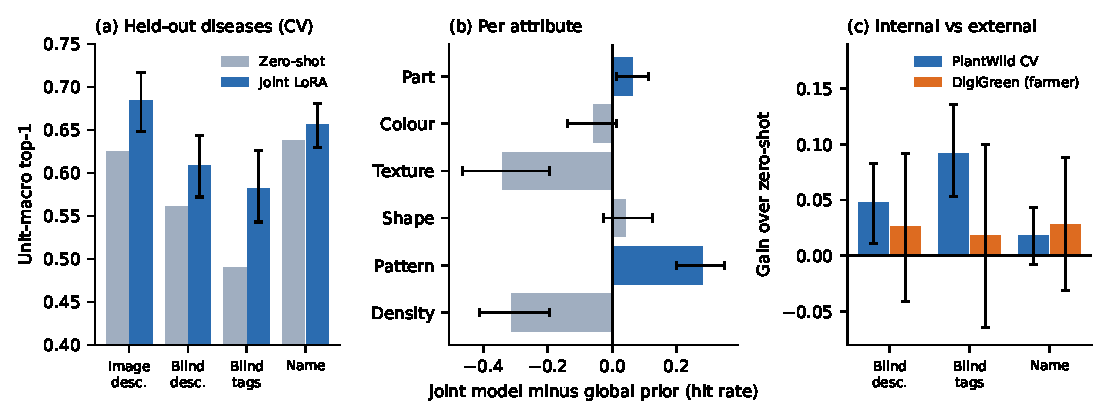
\includegraphics[width=\linewidth]{figures/results_summary.pdf}
\caption{Summary of the evidence (joint model, descriptions re-sampled; numbers from Tables~\ref{tab:joint}, \ref{tab:jointattr}, \ref{tab:jointdg}). (a) Held-out-disease top-1 in CV, zero-shot against joint LoRA; bars on the joint model show the 95\% interval of the gain, shifted onto the joint bar. (b) Joint model minus the global-prior hit rate per attribute; blue = interval above zero. (c) Gain over zero-shot in CV and on 423 farmer photos (39 types): the farmer-photo intervals include zero.}\label{fig:summary}
\end{figure}

\subsection{Unseen-disease generalisation on farmer photographs}\label{sec:dg}
\textbf{Small matched test.} Table~\ref{tab:dg} uses the 69 images of 14 diseases that match PlantWild units, scored with image-derived profiles of the matched PlantWild disease. The supervised model transfers: with symptom text only, 0.662 against 0.536 (+0.13). The three seeds agree, but there are only 69 images and 14 disease types, so the interval is about $\pm0.11$. This is the vision-only model; the joint model was trained without all matched diseases and was therefore evaluated on the large test only.
\begin{table}[t]\centering\small
\begin{tabular}{lcc}\toprule
Model (69 images, 14 unseen diseases) & Zero-shot & Supervised (3 seeds)\\\midrule
Symptom text only & 0.536 & 0.662 (0.667, 0.652, 0.667)\\
Symptom text + name & 0.536 & 0.686 (0.696, 0.696, 0.667)\\\bottomrule
\end{tabular}
\caption{DigiGreen top-1 with crop given; candidates are all units of the crop. The final training step is used (no validation set).}\label{tab:dg}
\end{table}

\textbf{Large test with blind profiles.} Table~\ref{tab:dgfull} uses 423 images of 39 disease types in 12 crops, scored with profiles written blind from the disease name. With the DigiGreen types of the crop as candidates, symptom-description scoring improves from 0.412 to 0.447 (seed std 0.002), a gain of +0.035 with a bootstrap interval over the 39 types of $[-0.025, 0.098]$ (14 types improved, 8 got worse); on the 34 types with no PlantWild counterpart the figures are 0.398 and 0.431. This is not distinguishable from zero. Adding the crop's PlantWild units as extra distractors removes the gain (0.352 to 0.342). Disease-name prompts are better than blind symptom profiles here (0.470, 0.533 after training), so on this test the symptom route does not beat the name route. Training on symptom text raises the name-prompt score too, which suggests that part of the improvement lies in the image features and not in the symptom--text match. A Qwen2.5-VL-7B zero-shot tagger reaches 0.312 and multiple choice by name 0.499 on the matched types (13 units).
\begin{table}[t]\centering\small
\resizebox{\linewidth}{!}{\begin{tabular}{llcccc}\toprule Scoring text & Candidates & Zero-shot & Supervised & Unmatched only (zs / sup.)\\\midrule
Blind symptom profile (description) & DigiGreen types & 0.412 & 0.447 $\pm$ 0.002 & 0.398 / 0.431\\
Blind symptom profile (description) & + PlantWild units & 0.352 & 0.342 $\pm$ 0.001 & 0.352 / 0.346\\
Blind symptom profile (tag list) & DigiGreen types & 0.397 & 0.413 $\pm$ 0.009 & 0.405 / 0.395\\
Blind symptom profile (tag list) & + PlantWild units & 0.314 & 0.321 $\pm$ 0.007 & 0.337 / 0.328\\
Disease-name prompt & DigiGreen types & 0.470 & 0.533 $\pm$ 0.004 & 0.496 / 0.528\\
Disease-name prompt & + PlantWild units & 0.424 & 0.431 $\pm$ 0.003 & 0.465 / 0.458\\
\bottomrule\end{tabular}
}
\caption{Large DigiGreen test (423 images, 39 types, 12 crops; types-macro top-1, crop given). Supervised: mean $\pm$ std over three seeds of the symptom-only training recipe, trained without any PlantWild unit that matches a DigiGreen disease. Profiles are written blind by an LLM from the disease name. ``Unmatched only'' = the 34 types with no PlantWild counterpart.}\label{tab:dgfull}
\end{table}

\textbf{Training on blind profiles, large test.} Table~\ref{tab:dgfullblind} adds models trained on blind profiles. For description scoring they are slightly below zero-shot (0.396 against 0.412; $-0.016$ over types, interval $[-0.091, 0.055]$, 15 types better and 13 worse); for names they improve (0.509 against 0.470). Neither training variant gives a reliable gain for symptom-profile scoring on this test, which includes pests and nutrient deficiencies that are far from PlantWild's training diseases.
\begin{table}[t]\centering\small
\resizebox{\linewidth}{!}{\begin{tabular}{llccc}\toprule Scoring text & Candidates & Zero-shot & Trained on image-derived & Trained on blind\\\midrule
Blind description & DigiGreen types & 0.412 & 0.447 $\pm$ 0.002 & 0.396 $\pm$ 0.005\\
Blind description & + PlantWild units & 0.352 & 0.342 $\pm$ 0.001 & 0.308 $\pm$ 0.007\\
Blind tag list & DigiGreen types & 0.397 & 0.413 $\pm$ 0.009 & 0.400 $\pm$ 0.004\\
Blind tag list & + PlantWild units & 0.314 & 0.321 $\pm$ 0.007 & 0.313 $\pm$ 0.002\\
Disease-name prompt & DigiGreen types & 0.470 & 0.533 $\pm$ 0.004 & 0.509 $\pm$ 0.002\\
Disease-name prompt & + PlantWild units & 0.424 & 0.431 $\pm$ 0.003 & 0.397 $\pm$ 0.002\\
\bottomrule\end{tabular}
}
\caption{Large DigiGreen test, types-macro top-1, three seeds (mean $\pm$ std). The two training columns differ only in the text used for the training diseases (image-derived tags or blind LLM profiles).}\label{tab:dgfullblind}
\end{table}

\section{Failure Analysis and Lessons}\label{sec:fail}
\subsection{Ablations in this protocol}\label{sec:abl}
The recipe is not the bottleneck: learning-rate, step-count, LoRA-placement and prompt variants all stay within fold noise (Appendix~\ref{app:recipe}).

\textbf{Synthetic lesion edits.} In the earlier experiments on the old 5-fold protocol (folds 2--5, v2 labels) colour, size, density and compositional edits, a paired loss, a patch head and LoRA with edits did not improve held-out-disease top-1 over real-only training (trained attribute heads: 0.4625 real-only against 0.439--0.456 with colour, LaMa, single-attribute or compositional edits; LoRA backbone on folds 2--4: 0.408 real-only against 0.381 with all edits). We therefore do not include synthetic data in the final model and do not claim it as a contribution. These numbers are from the previous protocol and are not directly comparable with Table~\ref{tab:main}.

\textbf{Name text.} Name-only supervised scoring on DigiGreen reaches about 0.60 after training, below description-only scoring (0.66), while the combination is best (0.686); before training both are about 0.52--0.54.

\subsection{Lessons from earlier experiments}\label{sec:lessons}
This paper is the end of a longer line of work: more than a hundred numbered experiments in the first version of the project and several dozen in the next three, all run on earlier protocols (class-family folds or frozen folds, other candidate sets and weightings) that we later replaced by the unit-grouped CV used here. Their numbers are therefore \emph{not} comparable with the tables above and are given only with their protocol (``v2'', ``v3'' and ``v5-old'' below); we report the findings that changed what we built or what we dare to claim, not every run.
\begin{table}[!htbp]\centering\small
\begin{tabular}{p{0.25\linewidth}p{0.45\linewidth}p{0.21\linewidth}}\toprule
Finding & Evidence (protocol) & Consequence \\\midrule
Class-level symptom labels are too noisy to learn from & Symptom nAP stayed at 0.24--0.30 for every encoder, head and fine-tune (v2); a blind per-image check found class priors agree with the photo for only 43\% (halo) to 80\% (border) of images & Per-image part and group-level symptom annotation (Section~\ref{sec:data}) \\
Names are not what the model learns from & Name-free caption retrieval 83.0 vs name prompts 82.6 on unseen diseases (v3); scrambling the name to a random code drops name matching to 0.285, close to crop-only text (0.306) (v5-old) & Name results mostly reflect pretraining; we never claim to beat names \\
The symptom text carries the signal & True profile 0.683, profile shuffled within the crop 0.119, crop-only text 0.306 (v5-old); 0.136 and 0.269 in the final protocol & Shuffled and crop-only controls are reported throughout \\
Colour and part matter most; texture and density add nothing to matching & Corrupting the profile of unseen diseases: dropping colour 0.542, part 0.625, pattern 0.634, shape 0.651 from 0.675; texture, size and density no effect (v5-old) & Consistent with our weak texture and density probes \\
Attribute heads plus lookup lose to frozen matching, and lookup is not the cause & Heads 0.463 vs frozen description 0.683, while looking up the true tags gives 1.000 (v5-old); 0.361 vs 0.627 in the final protocol; fusing both gives no gain & Description matching is the method; heads are a probe \\
Trained heads favour seen diseases & With about 150 candidates and no crop, a trained disease outranks the true held-out one in 83\% of failures (v5-old) & Crop given, candidates restricted to the crop \\
Most adaptation variants are inside noise & Mild and bold fine-tunes $+0.000$ to $+0.006$, contrast head $+0.006$, profile-matching loss $0.638\to0.630$ with validation up and test down (v5-old) & Only adapting both towers cleared noise (Section~\ref{sec:joint}) \\
Synthetic lesions do not help & Removing synthetic images $+0.012$ nAP; synthetic-only transfer 0.065 nAP (v2); real-only top-1 0.4625 vs 0.439--0.456 with edits, edits move the frozen embedding by only 0.032 in cosine (v5-old) & No synthetic data in the final model \\
Re-annotation improved trust, not accuracy & Frozen matching 0.666 with v2 labels, 0.638 with v3 raw value names and 0.650 with natural phrases; vocabulary merging alone costs about 0.016 (v5-old) & Annotation quality limits are reported, not hidden \\
The old split was unfair to some diseases & 17 of 70 test units had top-1 of 0, mostly near-identical siblings; one unit with 386 images was 18\% of a fold and shifted its macro-AP by 0.073 (v5-old) & Unit-grouped 10-fold CV with unit-macro scores \\
Crop recognition, not symptoms, dominated name accuracy & Giving the true crop raised name accuracy over all 89 classes from 8.6\% (no crop) and 18.3\% (predicted crop) to 62.6\%, and 80\% of errors were in the wrong crop (v2) & The crop is given at inference \\
Source shortcuts are easy to create & Nutrient-deficiency recall was 98.6\% on a controlled-capture coffee set but 0.9\% on PlantWild blossom-end rot (v2) & PlantWild-only evaluation; no controlled-capture data \\
\bottomrule\end{tabular}
\caption{Findings from earlier experiments that shaped the final design. Numbers use the protocol named in brackets (v2: class-family folds and nAP; v3: family folds, top-1; v5-old: frozen folds with held-out units) and are not comparable with the main tables. The v3 symptom-removal test (unseen top-1 51.5 with lesions removed against 72.7 for the original images, SigLIP2-b) was never repeated with a random-region control, so it shows that accuracy falls without lesions, not that lesions are the only cue.}\label{tab:lessons}
\end{table}

\subsection{Error analysis and limitations}\label{sec:limits}
\begin{itemize}
\item The joint model's cross-validation gains ($+0.048$ to $+0.092$ for descriptions) are not confirmed on the large DigiGreen test (intervals include zero), and the profile of a held-out disease in cross-validation is either built from its own images or written by an LLM from its name, not by an expert.
\item The image-to-symptom transfer result (Section~\ref{sec:transfer}) uses group-level labels, a coarse hit criterion, one seed and a linear head; for colour, texture and lesion density it only ties the global prior.
\item The vision-only gain over zero-shot retrieval is small on PlantWild (+0.019, not significant for symptom-only) and uneven: on folds 2, 3 and 6 the supervised model matches zero-shot (within 0.005), on folds 7 and 9 it is slightly below, and on fold 4 it is clearly below (0.777 against 0.847). Many failing diseases have a near-identical sibling in the same crop (for example apple black rot and scab), so profile ambiguity contributes to the errors; Section~\ref{sec:disc} shows that it explains only part of them.
\item The gain depends on how the held-out profile is produced. With LLM-written blind profiles and image-derived training the CV gain vanishes (0.563 to 0.563); training on blind profiles recovers a small gain (+0.022), but on the large DigiGreen test neither variant helps reliably (+0.035 and $-0.016$, intervals include zero). The per-attribute probe shows improvement over a prior only for the affected part. We therefore do \emph{not} claim that the vision-only model learned colour, texture, pattern or lesion density; in the disease-macro test the vision-only and joint models both improve part and pattern over the global prior but not texture or lesion density (Table~\ref{tab:jointattr}).
\item The matched DigiGreen test is small (69 images, 14 diseases, no validation set); the large test uses profiles written by an LLM of limited quality (agreement with our tags 0.27--0.93 depending on the attribute) and removes only diseases matched by name.
\item Labels are group level, noisy and LLM-assisted; in the CV, profiles built from image tags use the test images' own tags.
\item Baselines are our re-implementations on our splits, and the VLM numbers use at most 6 images per unit.
\item The pretrained text encoder may carry knowledge of disease names from web pretraining, which limits how symptom-grounded any name-based result can be; the symptom-only track removes names from our inputs but not from the encoder's pretraining.
\item Nutrient deficiencies, other non-infectious problems and early-stage symptoms, which motivate this work, are barely covered by our data (one deficiency unit in PlantWild, no stage labels) and are not evaluated at scale; the large DigiGreen test contains three nutrient-deficiency types with three images each (nine images, two of the three types ranked first), which is anecdotal.
\item Explainability and farmer-correction claims were not tested. Checkpoints are provided for the joint model (10 folds and the DigiGreen model, three seeds) and for the earlier seed-0 vision models.
\end{itemize}

\section{Discussion}\label{sec:disc}
\textbf{The central tension: symptoms or correlates?} Image-derived descriptions improve from 0.625 to 0.684, blind LLM descriptions from 0.561 to 0.609 and name prompts from 0.638 to 0.656, yet on farmer photographs no improvement is significant and names remain stronger. Two readings fit this. Either the models learn symptom features that transfer between diseases inside PlantWild but are too weakly grounded to survive the shift to farmer photographs, or they exploit information correlated with disease identity (crop appearance, web-source style, what the pretrained text encoder already knows about names). The per-attribute probes favour a partial answer: part and pattern transfer beyond priors, texture and density do not. Distinguishing the two readings needs controls we have not run, such as attribute-level supervision on independent photographs, text-only adaptation on the per-attribute test, and expert-written descriptions; we therefore treat this as the open question of the paper and not as a limitation to be noted in passing.

\textbf{What the failed experiments say.} Table~\ref{tab:failures} reads the negative results as evidence about the problem.
\begin{table}[t]\centering\small
\begin{tabular}{p{0.34\linewidth}p{0.58\linewidth}}\toprule
Observation & Interpretation \\\midrule
Hard negatives mostly hurt & Separating near-identical sibling diseases through negatives may be unstable when their profiles overlap. \\
LLM paraphrasing is worse & More natural language does not mean better visual grounding. \\
Synthetic lesion edits do not help & Changing appearance alone does not improve disease-level generalisation. \\
Texture and density transfer poorly & These attributes may be least consistently visible and least consistently labelled (group-level tags; blind-profile agreement 0.58 and 0.27). \\
Farmer-photo gains are inconclusive & Disease-disjoint gains inside PlantWild do not guarantee field-level improvement. \\\bottomrule
\end{tabular}
\caption{Negative and inconclusive results and what they suggest.}\label{tab:failures}
\end{table}

\textbf{How much of the error is profile ambiguity?} For each test unit we computed the similarity (mean attribute-wise Jaccard over the six attributes) between its image-derived profile and that of its nearest same-crop sibling, and related it to the unit's accuracy under the symptom-only vision LoRA (seeds 1 and 2, all folds; Table~\ref{tab:amb}, Figure~\ref{fig:amb}). Accuracy falls as the sibling gets closer (Spearman $\rho=-0.46$ for the adapted model and $-0.44$ for zero-shot, $n=116$ units), so ambiguity is real. But no two same-crop units have identical profiles on all six attributes, and the units with the lowest accuracy often have siblings that differ on three to five attributes (carrot cercospora against alternaria leaf blight: four attributes differ, accuracy 0.00; bell pepper bacterial spot against leaf spot: four differ, 0.05). Adaptation gains over zero-shot are small in every group ($+0.016$, $+0.013$ and $+0.057$, the last with only 13 units and a wide interval; Table~\ref{tab:amb}), so there is no sign that it works by resolving ambiguity. We read this as: part of the error is information missing from the descriptions, but a large part is the model failing to read attributes (colour, shape, texture and density) that do distinguish the diseases, in line with the per-attribute probes. A diagnosis with several plausible candidates, rather than a single answer, is the natural output for the near-identical group.
\begin{table}[t]\centering\small
\begin{tabular}{lcccc}\toprule Nearest same-crop sibling profile & Units & Zero-shot & Symptom LoRA & Chance\\\midrule
distinct (<0.5) & 59 & 0.741 & 0.757 [0.691, 0.819] & 0.290\\
similar (0.5-0.7) & 44 & 0.516 & 0.529 [0.448, 0.607] & 0.249\\
near-identical (>=0.7) & 13 & 0.483 & 0.540 [0.393, 0.689] & 0.227\\
\bottomrule\end{tabular}

\caption{Unit top-1 by similarity of the unit's profile to its nearest same-crop sibling (116 test units, mean over seeds 1 and 2; interval is a bootstrap over units). Thresholds on the similarity are our choice. Chance is the mean of 1/(number of same-crop units).}\label{tab:amb}
\end{table}
\begin{figure}[t]\centering
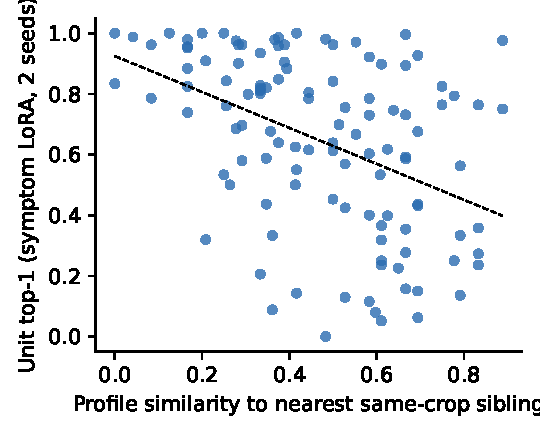
\includegraphics[width=0.55\linewidth]{figures/ambiguity.pdf}
\caption{Unit accuracy against profile similarity to the nearest same-crop sibling; dashed line is a least-squares fit.}\label{fig:amb}
\end{figure}

The picture across experiments is consistent in direction but modest in size. A head trained on seen diseases reads the affected part, shape and pattern of unseen diseases better than any prior, and adapting both towers of the matching model turns this into a reliable cross-validation gain over zero-shot retrieval, for texts that come from images and for texts written without seeing images. Adapting only one side (text-only LoRA gives $+0.031$, $+0.031$, $+0.075$, with the image-derived gain not significant), using hard negatives, other text encoders, LLM paraphrases or synthetic lesion edits gives smaller, non-significant or negative gains. Two things limit the claim. First, on a large independent set of farmer photographs with blind profiles the gains are about $+0.02$ to $+0.03$ and statistically indistinguishable from zero, and disease names remain a stronger signal there, partly because the pretrained text encoder already knows many names. Second, per attribute the adapted models beat the global prior only for part and pattern (and the crop prior also for shape); for colour, texture and lesion density they are no better, and for texture and density clearly worse, than predicting the most common value, and the joint model is not better than the vision-only model on these probes. We therefore read the evidence as support for symptom-level transfer of some attributes, not for a general ability to describe any new disease. The next steps are expert-written descriptions of new disorders, attribute-level supervision, better prompts or heads for texture and lesion density, and larger independent tests covering deficiencies, pests and early stages.

\textbf{Concerns a reader should raise, and where the paper stands.}
(1) \emph{Novelty.} We found no prior work that trains an image-to-symptom mapping and evaluates it on withheld diseases (Section~\ref{sec:related}); this is a statement about what we found, not a survey.
(2) \emph{Annotation quality.} Tags are group-level, mostly written by human annotators and partly by an LLM-assisted procedure (marked in the released file), and have no inter-annotator agreement statistic; the blind LLM profiles agree with our tags by 0.93 (part) down to 0.27 (density). Texture and density, the least reliable attributes, are also the ones models do not learn.
(3) \emph{Leakage.} Names never appear in symptom text; the crop is given; unit-level splits keep duplicates apart; DigiGreen diseases that match a PlantWild unit are removed from training; shuffled-text and shuffled-label controls collapse to or below chance. What we cannot exclude is crop or web-source style carrying disease identity, and name knowledge inside the pretrained encoder.
(4) \emph{Fair comparison.} All baselines run on the same splits, but they are our re-implementations, and the VLM baselines use at most six images per unit.
(5) \emph{External validity.} The farmer-photo test has 39 types, and its intervals (about $\pm0.07$) are wider than the gains ($+0.02$ to $+0.03$), so it is underpowered as well as inconclusive.
(6) \emph{Practical value.} A classifier cannot score a disease absent from its list, whereas this approach scores any disease for which a symptom description exists; on farmer photos, however, disease-name prompts are still stronger than symptom descriptions, so we do not claim the approach is yet better in practice.

\section{Conclusion}
We built symptom annotations, a strict unseen-disease protocol and a family of SigLIP2 models, and tested them with controls. A linear head shows that attribute values learned on seen diseases transfer to held-out diseases beyond crop and global priors for part, shape and pattern. A joint vision+text LoRA model improves held-out-disease matching over zero-shot by $+0.059$, $+0.048$ and $+0.092$ top-1 for image-derived, blind-description and blind-tag texts (three seeds, intervals above zero), while name prompts do not improve significantly. On a larger external farmer-photo test the gains are positive but not significant. The earlier vision-only results, shuffled-label and probe controls, and the negative synthetic-augmentation result are kept as context. Describing diseases that are in no dataset remains the main target of future work. We release the annotations, splits, code and checkpoints.

\appendix
\section{Recipe sweep}\label{app:recipe}
\textbf{Recipe sweep (symptom-only, folds 0,2,5,9, baseline 0.610).} A higher learning rate and 600 steps: 0.612; LoRA on all layers: 0.601; extra short prompt and cluster weight 1.0: 0.618; lower learning rate and 800 steps: 0.616. All are within fold noise, so the recipe is not the bottleneck.

\begin{thebibliography}{99}
\bibitem{clip} A.~Radford et al. Learning transferable visual models from natural language supervision. ICML, 2021.
\bibitem{siglip2} M.~Tschannen, A.~Gritsenko, X.~Wang, et al. SigLIP~2: Multilingual vision-language encoders with improved semantic understanding, localization, and dense features. arXiv:2502.14786, 2025.
\bibitem{lora} E.~J.~Hu et al. LoRA: Low-rank adaptation of large language models. ICLR, 2022 (arXiv:2106.09685).
\bibitem{mvpdr} T.~Wei, Z.~Chen, Z.~Huang, X.~Yu. Benchmarking in-the-wild multimodal plant disease recognition and a versatile baseline. ACM Multimedia, 2024 (arXiv:2408.03120; doi:10.1145/3664647.3680599).
\bibitem{snapn} T.~Wei, Z.~Chen, X.~Yu. Snap and Diagnose: An advanced multimodal retrieval system for identifying plant diseases in the wild. arXiv:2408.14723, 2024.
\bibitem{bcvsa} M.~R.~Hossain. BCVSA: Bias-calibrated visual-semantic alignment for generalized zero-shot plant disease recognition. Code repository (MIT license), github.com/RakibHossain011/BCVSA (accessed 2026).
\bibitem{mohanty2016} S.~P.~Mohanty, D.~P.~Hughes, M.~Salath\'e. Using deep learning for image-based plant disease detection. Frontiers in Plant Science 7:1419, 2016 (arXiv:1604.03169).
\bibitem{hughes2015} D.~P.~Hughes, M.~Salath\'e. An open access repository of images on plant health to enable the development of mobile disease diagnostics. arXiv:1511.08060, 2015.
\bibitem{xu2024} M.~Xu, J.-H.~Park, J.-H.~Lee, S.-H.~Yang, S.~Yoon. Plant disease recognition datasets in the age of deep learning: challenges and opportunities. Frontiers in Plant Science 15:1452551, 2024.
\bibitem{shoaib2023} M.~Shoaib et al. An advanced deep learning models-based plant disease detection: a review of recent research. Frontiers in Plant Science 14:1158933, 2023.
\bibitem{coleaf} V.~A.~Tuesta-Monteza, H.~I.~Mejia-Cabrera, J.~Arcila-Diaz. CoLeaf-DB: Peruvian coffee leaf images dataset for coffee leaf nutritional deficiencies detection and classification. Data in Brief 48:109226, 2023 (doi:10.1016/j.dib.2023.109226).
\bibitem{maizen} M.~Sala\'i\'c, F.~Novoselnik, I.~Podnar \v{Z}arko, V.~Gali\'c. Nitrogen deficiency in maize: annotated image classification dataset. Data in Brief 50:109625, 2023 (doi:10.1016/j.dib.2023.109625).
\bibitem{paddydoctor} A.~Petchiammal et al. Paddy Doctor: A visual image dataset for automated paddy disease classification and benchmarking. arXiv:2205.11108, 2022.
\bibitem{ccmt} P.~K.~Mensah et al. CCMT: Dataset for crop pest and disease detection. Data in Brief, 2023 (doi:10.1016/j.dib.2023.109306).
\bibitem{ip102} X.~Wu et al. IP102: A large-scale benchmark dataset for insect pest recognition. CVPR, 2019.
\bibitem{leafnet} K.~N.~Quoc, P.~D.~Dao, L.-D.~Quach. LeafNet: A large-scale dataset and comprehensive benchmark for foundational vision-language understanding of plant diseases. arXiv:2602.13662, 2026.
\bibitem{scold} K.~N.~Quoc, P.~D.~Dao, L.-D.~Quach. A vision-language foundation model for leaf disease identification. arXiv:2505.07019, 2025.
\bibitem{pvvqa} S.~N.~Sakib, N.~Haque, M.~Z.~Hossain, S.~E.~Arman. PlantExpertVQA: A visual question answering dataset for benchmarking vision-language models in plant science (first posted as PlantVillageVQA). arXiv:2508.17117, 2025.
\bibitem{plantseg} T.~Wei, Z.~Chen, X.~Yu, S.~Chapman, P.~Melloy, Z.~Huang. PlantSeg: A large-scale in-the-wild dataset for plant disease segmentation. arXiv:2409.04038, 2024.
\bibitem{zeng2024} Q.~Zeng, J.~Sun, S.~Wang. DIC-Transformer: interpretation of plant disease classification results using image caption generation technology. Frontiers in Plant Science 14, 2024 (doi:10.3389/fpls.2023.1273029).
\bibitem{agrogpt} M.~Awais et al. AgroGPT: Efficient agricultural vision-language model with expert tuning. WACV, 2025 (arXiv:2410.08405).
\bibitem{sage} M.~A.~Arshad, T.~Roy, Y.~Shen, D.~Elango, S.~Chiranjeevi, A.~K.~Singh, B.~Ganapathysubramanian, C.~Hegde, A.~Singh, S.~Sarkar. SAGE: Scalable agentic grounded evaluation for crop disease diagnosis. arXiv:2605.09768, 2026.
\bibitem{chatld} J.~Pan, R.~Zhong, F.~Xia, J.~Huang, L.~Zhu, Y.~Yang, T.~Lin. ChatLeafDisease: a chain-of-thought prompting approach for crop disease classification using large language models. Plant Phenomics 7:100094, 2025 (doi:10.1016/j.plaphe.2025.100094).
\bibitem{chai2024} A.~Y.~H.~Chai, S.~H.~Lee, F.~S.~Tay, P.~Bonnet, A.~Joly. Beyond supervision: Harnessing self-supervised learning in unseen plant disease recognition. Neurocomputing 610:128608, 2024 (doi:10.1016/j.neucom.2024.128608).
\bibitem{kumar2024} P.~Kumar, J.~Mathew, R.~K.~Sanodiya, T.~Setty, B.~P.~Bhaskarla. Zero shot plant disease classification with semantic attributes. Artificial Intelligence Review 57(11):305, 2024 (doi:10.1007/s10462-024-10950-9).
\bibitem{zhong2020} F.~Zhong, Z.~Chen, Y.~Zhang, F.~Xia. Zero- and few-shot learning for diseases recognition of Citrus aurantium L.\ using conditional adversarial autoencoders. Computers and Electronics in Agriculture 179:105828, 2020 (doi:10.1016/j.compag.2020.105828).
\bibitem{benabbas2025} Benabbas, Brahimi, Akhrouf, Fortas. Rethinking plant disease diagnosis: bridging the academic-practical gap with vision transformers and zero-shot learning. arXiv:2511.18989, 2025.
\bibitem{cupl} S.~Pratt, I.~Covert, R.~Liu, A.~Farhadi. What does a platypus look like? Generating customized prompts for zero-shot image classification. ICCV, 2023 (arXiv:2209.03320).
\bibitem{menon2023} S.~Menon, C.~Vondrick. Visual classification via description from large language models. ICLR, 2023 (arXiv:2210.07183).
\bibitem{lampert2014} C.~H.~Lampert, H.~Nickisch, S.~Harmeling. Attribute-based classification for zero-shot visual object categorization. IEEE TPAMI 36(3):453--465, 2014.
\bibitem{dinov2} M.~Oquab et al. DINOv2: Learning robust visual features without supervision. arXiv:2304.07193, 2023.
\bibitem{qwen} S.~Bai, K.~Chen, X.~Liu, et al. Qwen2.5-VL technical report. arXiv:2502.13923, 2025.
\bibitem{digigreen} Digital Green. Crop Disease Expert Annotations (989 farmer photographs with agronomist annotations, CC-BY-4.0). Hugging Face dataset DigiGreen/Crop\_Disease\_Images, 2026.
\bibitem{barbedo2016} J.~G.~A.~Barbedo. A review on the main challenges in automatic plant disease identification based on visible range images. Biosystems Engineering 144:52--60, 2016 (doi:10.1016/j.biosystemseng.2016.01.017).
\bibitem{dlcpd} H.-W.~Zhang, R.-F.~Wang, Z.~Wang, W.-H.~Su. DLCPD-25: A large-scale and diverse dataset for crop disease and pest recognition. Sensors 25(22):7098, 2025 (doi:10.3390/s25227098).
\end{thebibliography}
\end{document}
